% !TeX spellcheck = en_US

\chapter{Basics}
This chapter elaborates on the base technologies necessary to understand the following chapters.



\section{Related Work}
\cite{Wang2016} moving Obstacles



\section{MARS}
MARS (Multi-Agent Research and Simulation) is a working group at the HAW (University of applied Sciences) in Hamburg, Germany. The research group develops an distributed agent-based simulation system to be used by domain experts around the world. It consists of several components.


\subsection{LIFE}
The simulation system is called MARS LIFE. It executes simulation runs created inside the Cloud Services. For more detail see \cite{Huning2016}.


\subsection{Cloud Services}
The Cloud Services are the central back-end of the MARS system. These components are responsible for data import, persistence, data visualization an the connection between LIFE and the WebUI.


\subsection{WebUI}
The WebUI is the front-end of MARS. It is a web-based application that allows the user to control back-end services and trigger simulations from the web-browser.



\section{Geographic Information System (GIS)}
GIS contains of numerous technologies to store, manipulate, analyze and visualize geographical data. It can be used in all areas that need to work with spatial data. Some usages are the visualization of land-use, elevation data, weather maps, street networks and flood maps. To leverage the capabilities that GIS offers, specialized GIS software is required.


\subsection{Coordinate Reference System (CRS)}
In comparison to normal image data, GIS is usually geo-referenced, meaning each feature or pixel has a geospatial location. This is achieved by specific geo-aware formats that encode spatial positions into the data. This location is represented in a coordinate system. In GIS terminology this is referred to as \enquote{spatial reference system} (SRS) or \enquote{coordinate reference system} (CRS). Depending on the spatial area, coordinate systems provide different accuracy in their results. Some are optimized for certain areas, while others offer a general worldwide Accuracy.

\subsubsection{Mercator Projection}
The most globally used CRS is the Mercator projection. I was created by Gerardus Mercator in 1569 and has been improved over the years. Figure \ref{fig:mercator} shows the Mercator projection in it's normal and transverse orientation. The normal projection offers good general representation, while the transverse orientation is focuses on the poles.
\begin{figure}[H]
	\centering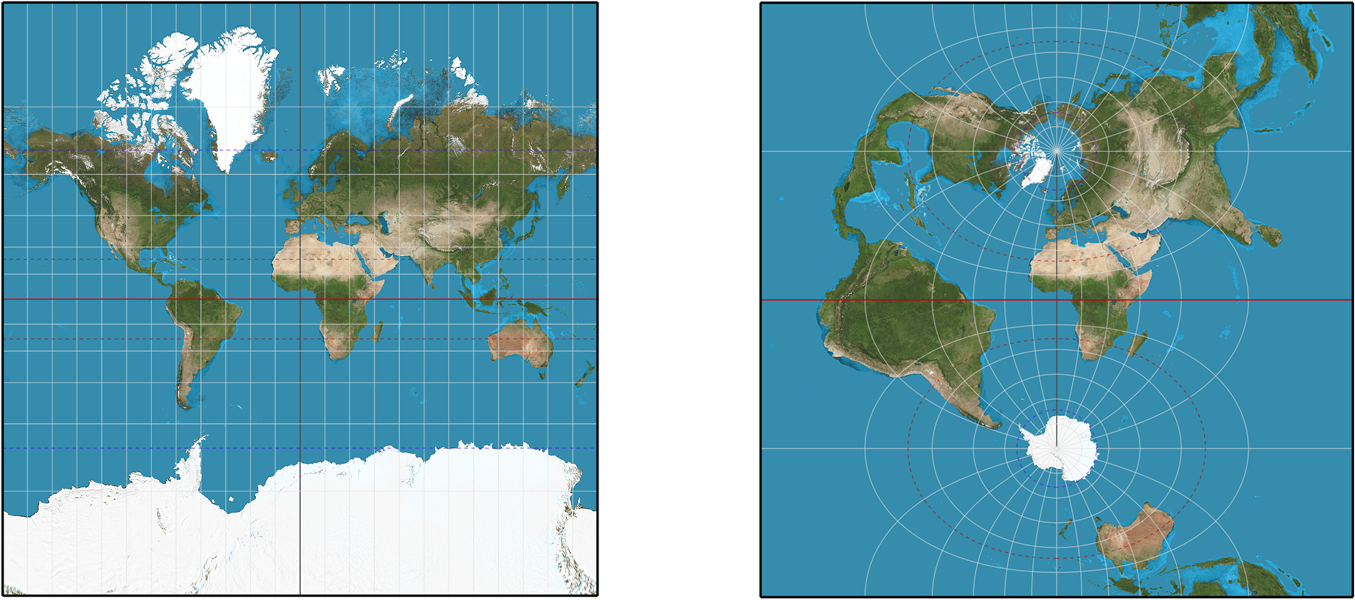
\includegraphics[width=1\textwidth]{res/Mercator}
	\caption{Normal and transverse Mercator projection. \url{https://commons.wikimedia.org/w/index.php?curid=9910866}}
	\label{fig:mercator}
\end{figure}

\subsubsection{EPSG:4326 -- WGS 84}
The most recent version of the Mercator projection is called WGS 84. It improves upon WGS 72 and is an \enquote{European Petroleum Survey Group} (EPSG) standard called EPSG:4326, created by \cite{Decker1986}.\\
WGS 84 is an ellipsoidal coordinate system that shows the 3D surface of the earth in 2D. The coordinates are longitude and latitude measured in degree. Longitude has the 0° point in Greenwich, England and increases east to a maximum of 180° and west to a minimum of -180°. Latitude has the 0° point at the equator and increases north to a maximum of 90° and south to a minimum of -90.\\
WGS 84 is used by the Global Positioning System (GPS), GIS specialists, inside the OpenStreetMap (OSM) database, as well as Google Earth.

\subsubsection{EPSG:3857 -- WGS 84 / Pseudo-Mercator}
Pseudo-Mercator is a projected version of WGS 84 into a cartesian coordinate system. The EPSG Standard is 3857 (EPSG:3857) by \cite{Grafarend1995}.\\
The CRS is based on a plane, rather then an ellipse. The zero points is identical to WGS 84 but the coordinates are X and Y measured in meters. The Y coordinate is limited to ±85.06° of the WGS 84 bounds. This results in a square projection with a range of ±20,026,376.39m on both axis, but sacrifices the poles to some extend. The square shape allow the creation of tile pyramids, also called \enquote{Mercator Pyramids}. \\
A pyramid is created, by cutting images of fixed size, usually 256px in width and height. Starting at one tile on the first zoom level, the amount of tiles is multiplied by four on every additional zoom level, to a maximum of around 18, depending on the implementation. \\
The resulting small images are optimal to be loaded on demand by a web browser. This is, why all major map sites, like OSM, Google Maps and Bing Maps use Pseudo-Mercator as their CRS. Figure \ref{img:mercator-pyramid} shows an example of a Mercator pyramid.
\begin{figure}[H]
	\centering
	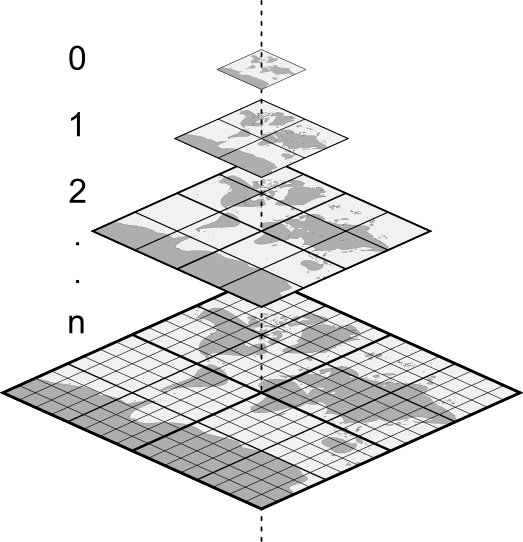
\includegraphics[width=0.4\columnwidth]{res/mercator-pyramid}\\
	\caption[]{Mercator tile pyramid. \url{http://data.webglearth.com/doc/webgl-earthch1.html}}
	\label{img:mercator-pyramid}
\end{figure}


\subsection{Spatial Data Types}
Geo-spatial data exist in two different types, vector and raster. 

\subsubsection{Raster Data}
 Raster data consists of a grid matrix in variable size.  Each grid cell is square and filled with a numeric value. The values can be encoded as color (e.g. satellite data) or as simple numeric values (e.g. elevation maps).  \\
 The advantage of raster data is that it can store any kind of GIS. The disadvantages are big files and the fixed pixel resolution which can not be changed after creation. Figure \ref{img:raster} shows a shape in three different raster resolutions, visualizing the loss of detail on lower raster resolutions.
 \begin{figure}[H]
 	\centering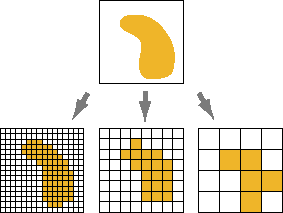
\includegraphics[width=.5\textwidth]{res/Vector-Raster}
 	\caption{Shape as raster in different resolutions. \url{http://desktop.arcgis.com/en/arcmap/latest/manage-data/raster-and-images/what-is-raster-data.htm}}
 	\label{img:raster}
 \end{figure}

\subsubsection{Vector Data}
Vector GIS has a much smaller file size, but is limited in its capabilities. It stores information based on mathematical functions. This is very efficient, but it is not suited for image like data such as land-use or elevation maps.\\
Data inside vector GIS can have several layers. Each layer can be of the type points, line or polygon. The data on a layer is called a feature. A point feature has a single coordinate, like a well. lines are open polygon lines and are often used for rivers. Shapes are closed lines and are used for areas like countries, lakes, or larger objects. See figure \ref{img:vector} for an example. \\
\begin{figure}[H]
	\centering
	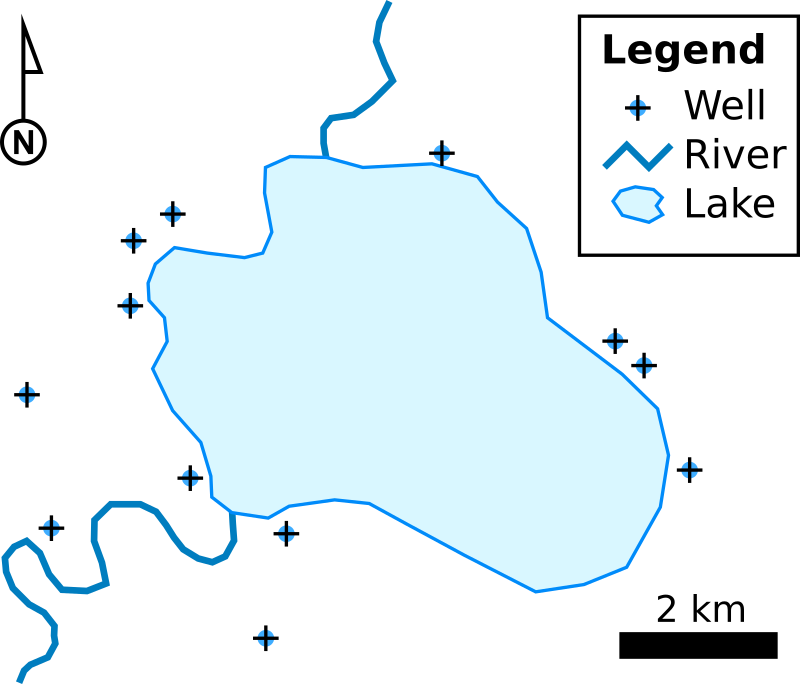
\includegraphics[width=0.4\columnwidth]{res/vector-map}\\
	\caption[]{Vector map with point, line and polygon. \url{https://commons.wikimedia.org/w/index.php?curid=3024482}}
	\label{img:vector}
\end{figure}



%\section{Mono}
%Open C\# implementation for Linux and OSX.
%
%
%
%\section{.NET Core}
%Microsoft bought Xamarin, which mostly developed Mono and is creating it's new C\# with build in multi-platform support.